\section{Motivation}

\begin{frame}\frametitle{Data Interoperability}
\begin{blockitems}{Situation}
 \item languages systems focus on different aspects
  \lec{frequent need to exchange data}
 \item generally, lots of aspect/language-specific objects
  \lec{proofs, programs, tables, sentences}
 \item but same/similar \emph{primitive} data types used across systems
  \lec{should be easy to exchange}
 \end{blockitems}
 
\begin{blockitems}{Problem}
 \item crossing system barriers usually require interchange language
  \lec{serialize as string and reparse}
 \item interchange languages typically untyped
  \lec{XML, JSON, YAML, \ldots}
\end{blockitems}

\begin{blockitems}{Solution}
 \item standardize primitive data types
 \item standardize encoding in interchange languages
\end{blockitems}
\end{frame}

\begin{frame}{Breakout Question}
What types do we need?
\end{frame}

\begin{frame}\frametitle{What types do we need?}
Focus on concrete types
\begin{itemize}
\item basic atomic types
\item collection and aggregation types
\item maybe some inductive data types?
\end{itemize}
\end{frame}

\begin{frame}\frametitle{Primitive vs. Declared}
\begin{blockitems}{Primitive Types}
 \item built into the language
 \item assumed to exist a priori \lec{fundamentals of nature}
 \item fixed semantics (usually interpreted by identity function)
 \end{blockitems}
 
\begin{blockitems}{Triple Structure: 3 kinds of named objects}
 \item the type \glec{eg: 'int'}
 \item values of the type \glec{eg: 0, 1, -1, \ldots}
 \item operations on type \glec{eg: addition, multiplication, \ldots}
\end{blockitems}

\begin{center}
\begin{tabular}{l|ll}
& primitive & declared \\
\hline
introduced by & language designer & user \\
introduced in & grammar & vocabulary $V$ \\
visible in & all vocabularies & $V$ only \\
semantics given & explicitly & implicitly \\
\tb\ldots by & translation function & axioms \\
\end{tabular}
\end{center}
\end{frame}

\begin{frame}\frametitle{Examples}
\begin{blockitems}{Typical primitive types}
 \item natural numbers (= $\N$)
 \item arbitrary precision integers (= $\Z$)
 \item fixed precision integers (32 bit, 64 bit, \ldots)
 \item floating point (float, double, \ldots)
 \item Booleans
 \item characters (ASCII, Unicode)
 \item strings
\end{blockitems}

Observation:
\begin{itemize}
\item essentially the same in every language
 \lec{including whatever language used for semantics}
\item semantics by translation trivial
\end{itemize}
\end{frame}

\begin{frame}\frametitle{Quasi-Primitive = Declared in standard library}
\begin{blockitems}{Standard library}
 \item present in every language
  \glec{assumed empty vocabulary by default}
 \item one fixed vocabulary
  \begin{itemize}
  \item implicitly included into every other vocabulary
  \item implicitly fixed by any translation between vocabularies
  \end{itemize}
 \item objects technically declared
 \item but practically part of primitive objects
\end{blockitems}

\begin{blockitems}{Examples}
\item sufficiently expressive languages
 \begin{itemize}
 \item push many primitive objects to standard library \glec{never all}
 \item simplifies language, especially when defining operations
 \end{itemize}
 \lec{strings in C, BigInteger in Java, inductive type for $\N$}
\item inexpressive languages
\begin{itemize}
\item many primitives \lec{SQL, spreadsheet software}
\item few (quasi)-primitives \lec{few operations available in OWL}
\end{itemize}
\end{blockitems}
\end{frame}

\begin{frame}\frametitle{Treatment in this Course}
\begin{blockitems}{BOL syntax and semantics so far}
\item primitive objects omitted in syntax
\item assumed reasonable collection available
\item assumed same (quasi-)primitive objects in semantic languages
 \lec{irrelevant if interpreting primitive objects as primitive or quasi-primitive}
\end{blockitems}
\lec{largely justified by practical languages}

\begin{blockitems}{But what exactly is the standard?}
\item will present possible solution
\item uses special ontology language just for specifying primitive objects
  \begin{itemize}
   \item name
   \item type
   \item semantics
    \glec{typically narrative; alternatively deductive, computational}
  \end{itemize}
\item current research, not standard practice
\end{blockitems}
\end{frame}

\begin{frame}\frametitle{Encoding Primitive Types}
\begin{blockitems}{Problem}
 \item quickly encounter primitive types not supported by common languages
 \item need to encode them using existing types
  \lec{typically as strings, ints, or prodcuts/lists thereof}
\end{blockitems}

\begin{blockitems}{Examples}
\item date, time, color, location on earth
\item graph, function
\item picture, audio, video
\item physical quantities ($1m$, $1in$, etc.)
\item gene, person
\end{blockitems}

\begin{center}
Breakout questions: What primitive types do we need for univis?
\end{center}
\end{frame}

\begin{frame}\frametitle{Failures of Encodings}
\begin{blockitems}{Y2K bug}
\item date encoded as tuple of integers, using $2$ digits for year
\item needed fixing in year 2000
\item estimated $\$300$ billion spent to change software
\item possible repeat: in 2038, number of seconds since 1970-01-01 (used by Unix to encode time as integer) overflows 32-bit integers
\end{blockitems}

\begin{blockitems}{Genes in Excel}
 \item 2016 study found errors in 20\% of spreadsheets accompanying genomics journal papers
 \item gene names encoded as strings but auto-converted to other types by Excel
 \begin{itemize}
 \item "SEPT2" (Septin 2) converted to September 02
 \item REKIN identifiers, e.g., "2310009E13", converted to float $2.31E+1$
 \end{itemize}
 \glec{\url{https://genomebiology.biomedcentral.com/articles/10.1186/s13059-016-1044-7}}
\end{blockitems}
\end{frame}

\begin{frame}\frametitle{Failures of Encodings (2)}
\begin{blockitems}{Mars Climate Orbiter}
\item two components exchanged physical quantity
\item specification required encoding as number using unit Newton seconds
\item one component used wrong encoding (with pound seconds as unit)
\item led to false trajectory and loss of $\$300$ million device
\end{blockitems}

\begin{blockitems}{Shellshock}
\item bash allowed gaining root access from 1998 to 2014
\item function definitions were encoded as source code
\item not decoded at all; instead, code simply run (as root)
\item allowed appending "; ..." to function definitions
\end{blockitems}
\lec{SQL injection similar: complex data encoded as string, no decoding}

\end{frame}

\begin{frame}\frametitle{Research Goal for Aspect-Independent Data in Tetrapod}
\begin{blockitems}{Standardization of Common Data Types}
 \item Ontology language optimized for declaring types, values, operations
 \glec{semantics must exist but can be extra-linguistic}
 \item Vocabulary declaring such objects
 \glec{should be standardized, modular, extensible}
\end{blockitems}

\begin{blockitems}{Standardization of Codecs}
\item Fixed small set of primitive objects
 \glec{should be (quasi-)primitive in every language}
 \glec{not too expressive, possibly untyped}
\item Standard codecs for translating common types to interchange languages
\end{blockitems}

\begin{blockitems}{Codec for type $A$ and int. lang. $L$}
\item coding function $A$-values $\to$ $L$-objects
\item partial decoding function $L$-objects $\to$ $A$-values
\item inverse to each other \glec{in some sense}
\end{blockitems}
\end{frame}

\begin{frame}\frametitle{Overview}
Next steps
\begin{enumerate}
\item Data types
\item Data interchange languages
\item Codecs
\end{enumerate}
\end{frame}

\section{Data Types}

\begin{frame}\frametitle{A Basic Language for Typed Data}
Let BDL be given by
\begin{commgrammar}
\gcomment{Types}\\
\gprod{T}{int \bnfalt float \bnfalt string \bnfalt bool}{base types}\\
\galtprod{\cn{list}\,T}{homogeneous lists}\\
\galtprod{\rep{(\ID:T)}}{record types}\\
\galtprod{\ldots}{additional types}\\
\gcomment{Data}\\
\gprod{D}{(64\, bit\, integers)}{}\\
\galtprod{(IEEE\, double)}{}\\
\galtprod{"(Unicode\, strings)"}{}\\
\galtprod{\cn{true} \bnfalt \cn{false}}{}\\
\galtprod{\rep{D}}{lists}\\
\galtprod{\rep{(\ID=D)}}{records}\\
\galtprod{\ldots}{constructors for additional types}\\
\end{commgrammar}
\end{frame}

\begin{frame}\frametitle{BDL Extended with Named ADTs}\label{def:bdl+adt}
\begin{commgrammar}
\gprod{V}{\rep{Decl}}{Vocabularies}\\
\gprod{Decl}{\kw{adt}\,t\,\{\rep{\ID:T}\}}{ADT definitions}\\
\galtprod{\kw{datum}\,d:T=D}{data definitions}\\
\gcomment{Types}\\
\gprod{T}{\ldots}{as before}\\
\galtprod{t}{reference to a named ADT}\\
\gcomment{Data}\\
\gprod{D}{\ldots}{as before}\\
\galtprod{d}{reference to a named datum}\\
\galtprod{t\{\rep{(\ID=D)}\}}{ADT elements}\\
\end{commgrammar}
\end{frame}


\section{Data Representation Languages}

\begin{frame}\frametitle{Overview}
\begin{blockitems}{General Properties}
 \item general purpose or domain-specific
 \item typed or untyped
  \lec{typical: Church-typed but no type operators, quasi untyped}
 \item text or binary serialization
 \item libraries for many programming languages
  \begin{itemize}
  \item data structures
  \item serialization (data structure to string)
  \item parsing (string to data structure, partial)
  \end{itemize}
\end{blockitems}

\begin{blockitems}{Candidates}
 \item XML: standard on the web, notoriously verbose
 \item JSON: JavaScript objects, more human-friendly text syntax
  \lec{older than XML, probably better choice than XML in retrospect}
 \item YAML: line/indentation-based
\end{blockitems}
\end{frame}

\begin{frame}{Breakout Question}
What is the difference between JSON, YAML, XML?
\end{frame}

\begin{frame}\frametitle{Typical Data Representation Languages}
XML, JSON, YAML essentially the same
 \lec{except for concrete syntax}

\begin{blockitems}{Atomic Types}
 \item integer, float, boolean, string
 \item need to read fine-print on precision
\end{blockitems}
 
\begin{blockitems}{(Not Very) Complex Types}
 \item heterogeneous lists
  \glec{a single type for all lists}
 \item records
  \glec{a single type for all records}
\end{blockitems}
\end{frame}

\begin{frame}\frametitle{Example: JSON}
JSON:
\[\mathll{
 \{\\
 \tb "individual": "Florian Rabe",\\
 \tb "age": 40,\\
 \tb "concepts": ["instructor", "male"],\\
 \tb "teach": [\\
 \tb\tb\{"name":"Wuv",credits:7.5\},\\
 \tb\tb\{"name":"KRMT",credits:5\}\\
 \tb]\\
\}
}\]


Weirdnesses:
\begin{itemize}
\item atomic/list/record = basic/array/object
\item record field names are arbitrary strings, must be quoted
\item records use $:$ instead of $=$
\end{itemize}
\end{frame}

\begin{frame}\frametitle{Example: YAML}
inline syntax: same as JSON but without quoted field names

alternative: indentation-sensitive syntax
\[\mathll{
 individual: "Florian Rabe"\\
 age: 40\\
 concepts:\\
 \tb  -\; "instructor"\\
 \tb  -\; "male"\\
 teach:\\
 \tb -\; name: "WuV"\\
 \tb\phantom{-}\; credits: 7.5\\
 \tb  -\; name: "KRMT"\\
 \tb\phantom{-}\; credits: 5\\
}\]

Weirdnesses:
\begin{itemize}
\item atomic/list/record = scalar/collection/structure
\item records use $:$ instead of $=$
\end{itemize}
\end{frame}

\begin{frame}[fragile]\frametitle{Example: XML}
Weird structure but very similar
\begin{itemize}
\item elements both record (= attributes) and list (= children)
\item elements carry name of type (= tag)
\end{itemize}

\begin{lstlisting}[basicstyle=\footnotesize]
<Person individual="Florian Rabe" age="40">
 <concepts>
   <Concept>instructor</Concept/>
   <Concept>male</Concept/>
 </concepts>
 <teach>
   <Course name="WuV" credits="7.5"/>
   <Course name="KRMT" credits="5"/>
 </teach>
</Person>
\end{lstlisting}

\begin{itemize}
\item Good: \lstinline|Person|, \lstinline|Course|, \lstinline|Concept| give type of object
 \glec{easier to decode}
\item Bad: value of record field must be string
 \glec{concepts cannot be given in attribute}
 \glec{integers, Booleans, whitespace-separated lists coded as strings}
\end{itemize}
\end{frame}

\begin{frame}\frametitle{Structure Sharing}
\begin{blockitems}{Problem}
\item Large objects are often redundant
 \glec{specially when machine-produced}
\item Same string, URL, mathematical objects occurs in multiple places
\item Handled in memory via pointers
\item Size of serialization can explode
\end{blockitems}

\begin{blockitems}{Solution 1: in language}
\item Add definitions to language
 \glec{common part of most languages anyway}
\item Users should introduce name whenever object used twice
\item Problem: only works if 
 \begin{itemize}
  \item duplication anticipated
  \item users introduced definition
  \item duplication within same context
   \glec{structure-sharing most powerful if across contexts}
 \end{itemize}
\end{blockitems}
\end{frame}

\begin{frame}\frametitle{Structure Sharing (2)}
\begin{blockitems}{Solution 2: in tool}
\item Use factory methods instead of constructors
\item Keep huge hash set of all objects
\item Reuse existing object if already in hash set
\item Advantages
 \begin{itemize}
  \item allows optimization
  \item transparent to users
 \end{itemize}
\item Problem: only works if 
 \begin{itemize}
  \item for immutable data structures
  \item if no occurrence-specific metadata \glec{e.g., source reference}
 \end{itemize}
\end{blockitems}

\begin{blockitems}{In data representation language}
\item Allow any subobject to carry identifier
\item Allow identifier references as subobjects
\lec{allows preserving structure-sharing in serialization}
\end{blockitems}
\lec{supported by XML, YAML}
\end{frame}

\section{Codecs}

\begin{frame}\frametitle{General Definition}
Throughout this section, we fix a data representation language $L$.
\lec{$L$-words called codes}

Given a data type $T$, a codec for $T$ consists
\begin{itemize}
 \item coding function: $c:T \to L$
 \item partial decoding function: $d:L\to^? T$
 \item such that
  \[d(c(x))=x\]
\end{itemize}
\end{frame}

\begin{frame}\frametitle{Codec Operators}
Given a data type operator $T$ taking $n$ type arguments,\\
a codec operator $C$ for $T$
\begin{itemize}
 \item takes $n$ codecs $C_i$ for $T_i$
 \item returns a codec $C(C_1,\ldots,C_n)$ for $T(T_1,\ldots,T_n)$
\end{itemize}
\end{frame}

%\begin{frame}\frametitle{Exercise 4}
%We fix strings as the data representation language $L$.
%
%Then, 
%\begin{enumerate}
% \item Jointly specify
%  \begin{itemize}
%  \item additional BDL types and constructors for univis-specific data
%  \item codecs and codec operators for all types resp. type operators
%  \end{itemize}
% \item Individually, in any programming language, implement
%  \begin{itemize}
%   \item data structures for BDL
%   \item string codecs (operators) for all BDL base types (operators)
%  \end{itemize}
% \item Use your codecs to exchange example data with your fellow students, who used different implementations and different programming languages.
%\end{enumerate}
%\end{frame}

\begin{frame}\frametitle{Codecs for Base Types}
We define codecs for the base types using strings as the data representation language $L$.

Easy cases:
\begin{itemize}
\item StandardFloat: as specified in IEEE floating point standard
\item StandardString: as themselves, quoted
\item StandardBool: as $true$ or $false$
\item StandardInt (64-bit): decimal digit-sequences as usual
\end{itemize}
\end{frame}

\begin{frame}\frametitle{Breakout Question}
How to encode unlimited precision integers?
\end{frame}

\begin{frame}\frametitle{Codecs for Unlimited Precision Integers}
Encode $z\in\Z$
\begin{itemize}
\item $L$ is strings: decimal digit sequence as usual
\item $L$ is JSON:
 \begin{itemize}
 \item IntAsInt: decimal digit sequence as usual
   \glec{JSON does not specify precision}
   \glec{but target systems may get in trouble}
 \item IntAsString: string containing decimal digit sequence
   \glec{safe but awkward}
 \item IntAsDecList: list of decimal digits
   \glec{safe but awkward}
 \item IntAsList1: as list of digits for base $2^{64}$
   \glec{OK, but we can do better}
 \item IntAsList2: as list of
   \begin{itemize}
   \item integer for the number of digits, sign indicate sign of $z$
   \item list of digits of $|z|$ for base $2^{64}$
   \end{itemize}
   Question: Why is this smart?
   
   \onslide<2>{Can use lexicographic ordering for size comparison}
 \end{itemize}
\end{itemize}
\end{frame}

\begin{frame}\frametitle{Codecs for Lists}
Encode list $x$ of elements of type $T$
\begin{itemize}
\item $L$ is strings: e.g., comma-separated list of $T$-encoded elements of $x$
\item $L$ is JSON:
 \begin{itemize}
 \item ListAsString: like for strings above
 \item ListAsArray: lists JSON array of $T$-encoded elements of $x$
 \end{itemize}
\end{itemize}
\end{frame}


\begin{frame}\frametitle{Additional Types}
Examples: semester

Extend BDL:
\begin{commgrammar}
\gcomment{Types}\\
\gprod{T}{Sem}{semester}\\
\gcomment{Data}\\
\gprod{D}{sem(int, bool)}{i.e., year + summer$^?$}\\
\end{commgrammar}

Define standard codec:
\[sem(y,true) \rewrites "SSY"\]
\[sem(y,false) \rewrites "WSY"\]
where $Y$ is encoding of $y$
\end{frame}

\begin{frame}\frametitle{Additional Types (2)}
Examples: timestamps

Extend BDL:
\begin{commgrammar}
\gcomment{Types}\\
\gprod{T}{timestamp}{}\\
\gcomment{Data}\\
\gprod{D}{\text{(productions for dates, times, etc.)}}{}
\end{commgrammar}

Standard codec: encode as string as defined in ISO 8601
\end{frame}

%%%%%%%%%%%%%%%%%%%%%%%%%%%%%%%%%%%%%%%%%%%%%%%%%%%%%%%%%%%%%%%%%%%%%%%%%%%%%%%%%%%%%%%%%%
\section{Data Interchange}

\begin{frame}\frametitle{Design}
\begin{enumerate}
\item Specify type system, e.g., BDL
 \begin{itemize}
 \item types
 \item constructors
 \item operations
 \end{itemize}
 \glec{can be done in appropriate type theory}
\item Pick data representation language $L$
\item Specify codecs for type system and $L$
 \begin{itemize}
 \item at least one codec per base type
 \item at least one codec operator per type operator
 \end{itemize}
 \glec{on paper}
\item Every system implements
 \begin{itemize}
 \item type system (as they like)
  \glec{typically aspect-specific constraints}
 \item codecs as specified
 \item function mapping types to codecs
 \end{itemize}
\item Systems can exchange data by encoding-decoding
 \lec{type-safe because codecs chosen by type}
\end{enumerate}
\end{frame}

\begin{frame}\frametitle{Example}
Implementation in Scala part of course resources
\end{frame}

\begin{frame}\frametitle{Example Application: OpenDreamKit research project}
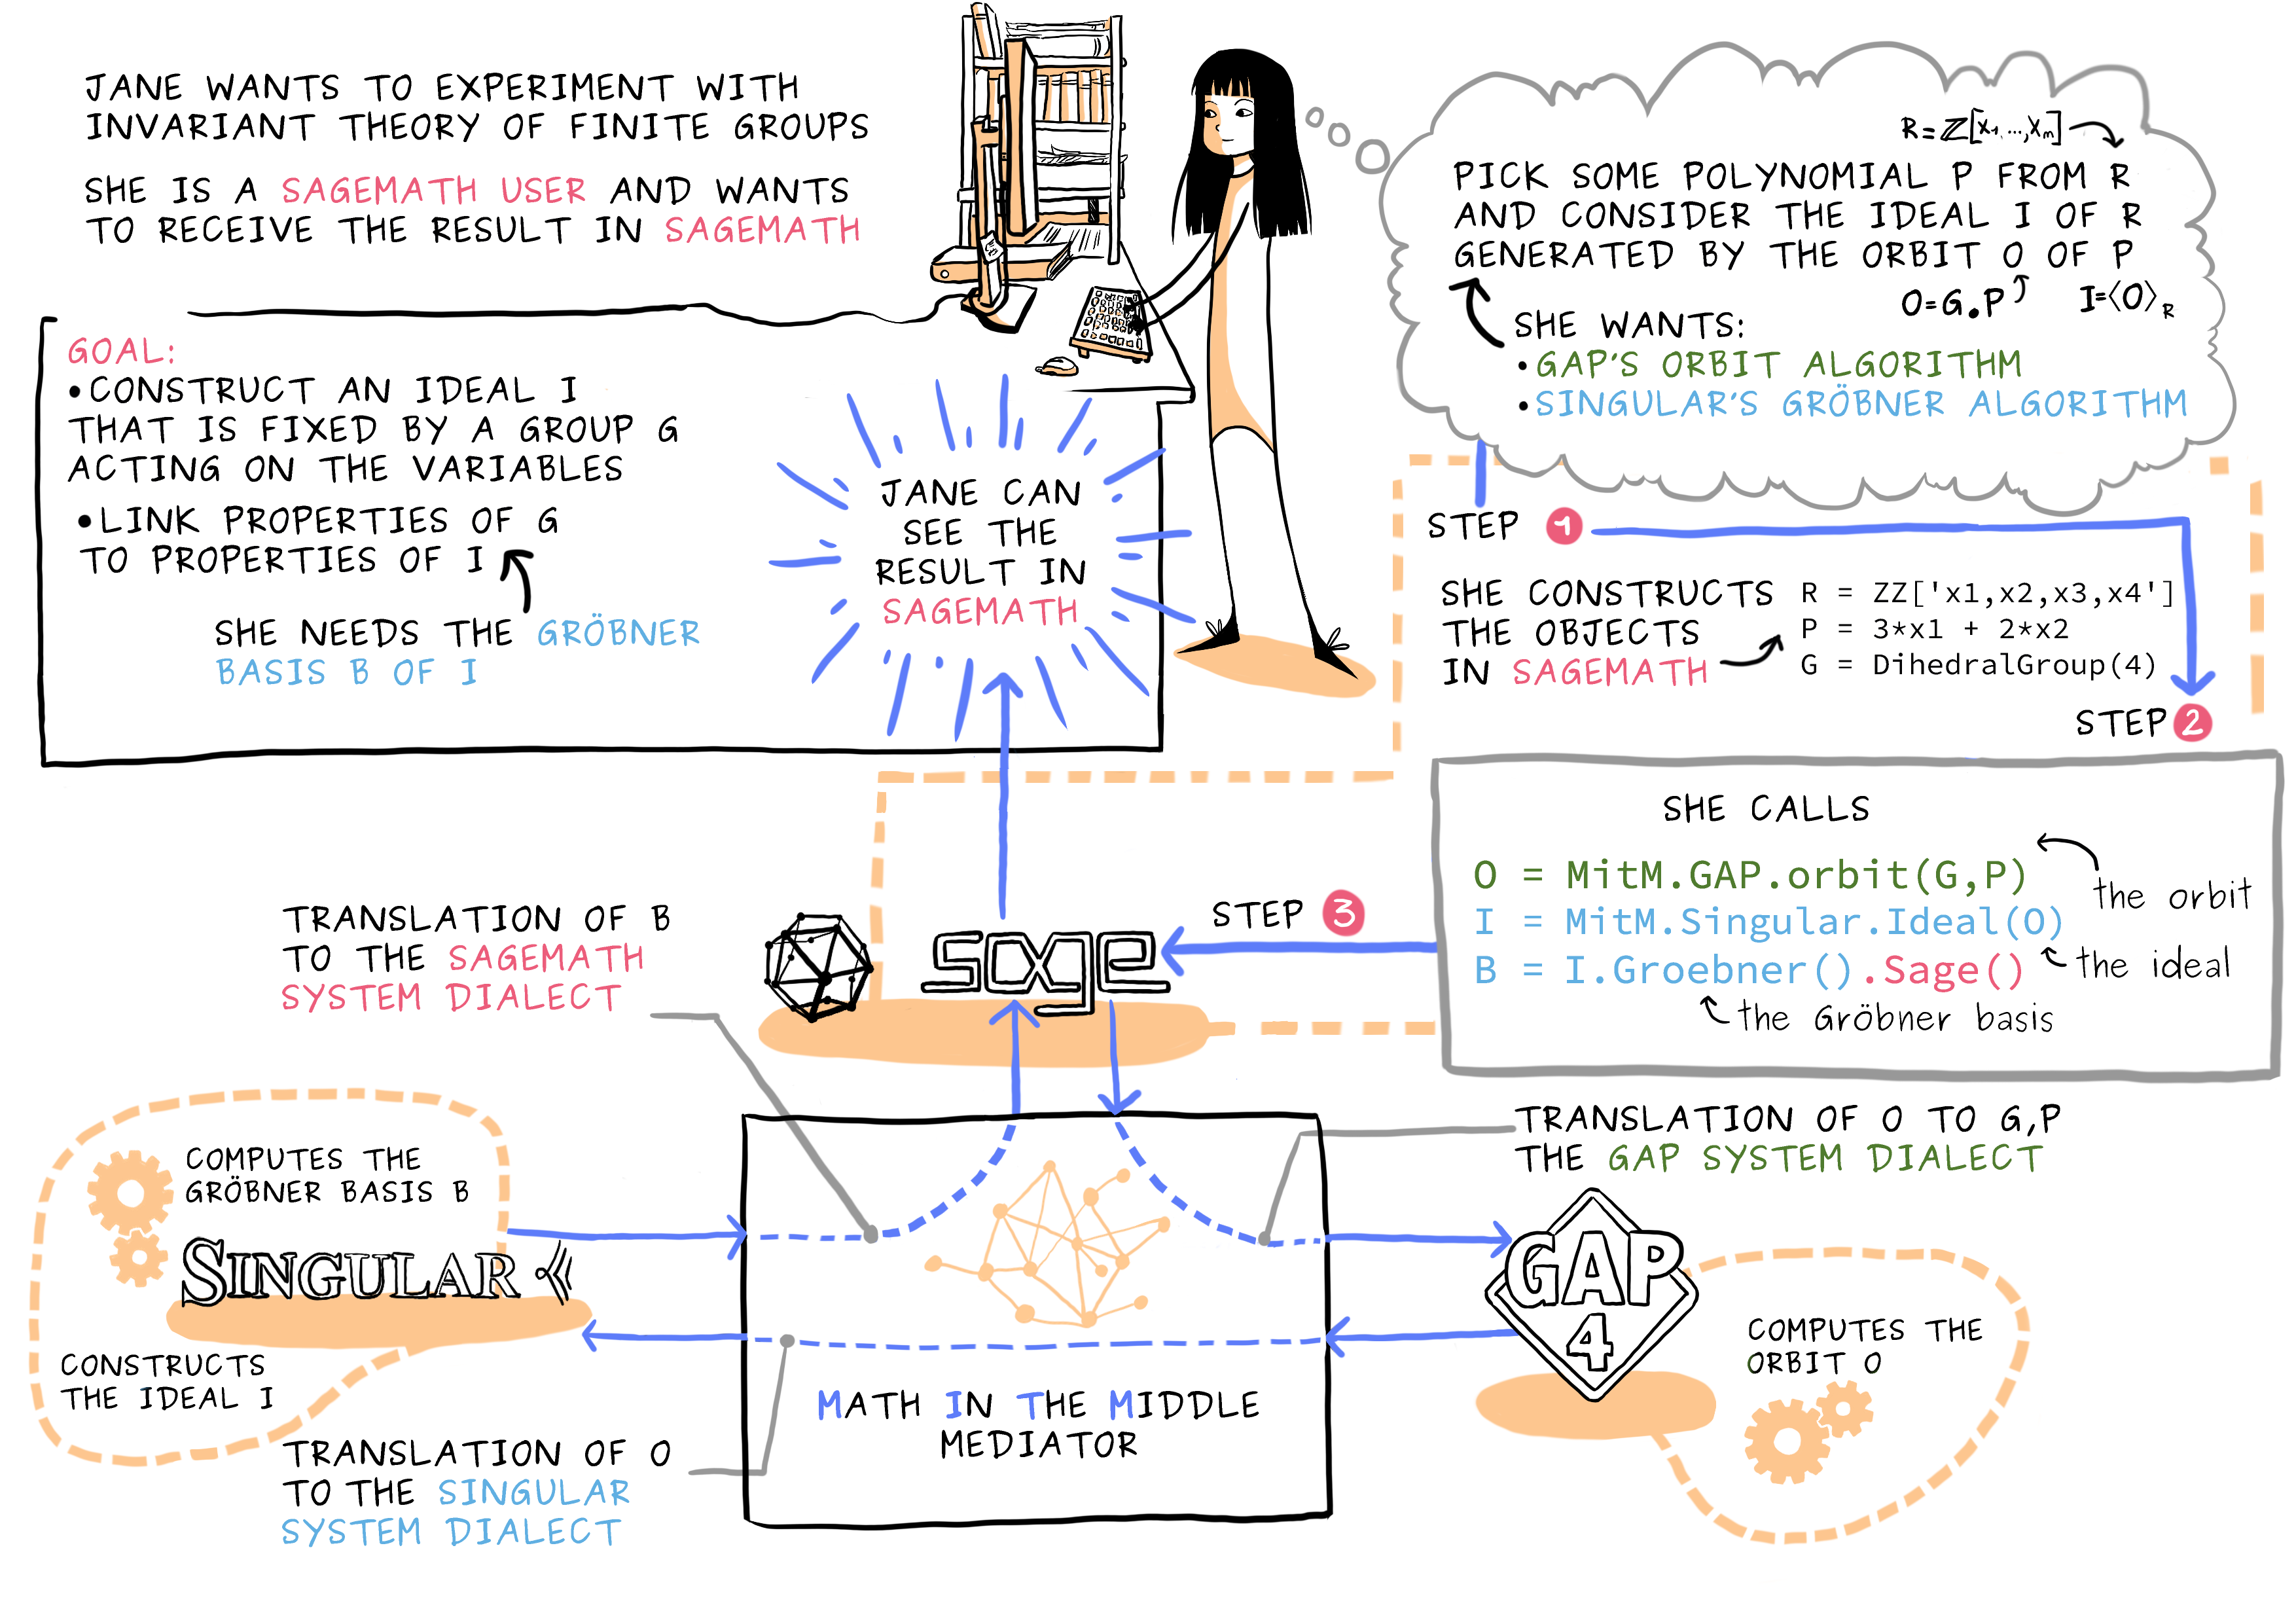
\includegraphics[width=\textwidth]{MitM.png}
\end{frame}

\begin{frame}\frametitle{Integrating BOL and BDL}
\begin{blockitems}{OWL-near option}
\item use BDL to define the primitive types of BOL
\item use those as types of BOL properties
\item Curry-typing throughout
\lec{easy: just merge the grammars}
\end{blockitems}

\begin{blockitems}{SQL-near option}
\item use BDL to define the primitive types of BOL
\item also add ADTs
\item Church typing more prominent
\lec{open question: ADTs in addition to or instead of BOL concepts}
\end{blockitems}

We assume the latter for now without spelling out the details.
\end{frame}

\begin{frame}\frametitle{BDL-Mediated Interoperability}
Idea
 \begin{itemize}
 \item define data types in BDL \glec{or similar typed ontology language}
 \item use ADTs
 \item generate corresponding
  \begin{itemize}
  \item class definitions for programming languages PL
   \lec{one class per ADT}
  \item table definitions in SQL
   \lec{one table per ADT}
  \end{itemize}
 \item use codecs to convert automatically when interchanging data between PL and SQL
 \end{itemize}

Open research problem
 \lec{no shiny solution yet that can be presented in lectures}
\end{frame}

\begin{frame}\frametitle{Codecs in ADT Definitions}
\begin{blockitems}{SQL table schema = list of fields where field is}
\item name
\item type \glec{only types of database supported}
\end{blockitems}

\begin{blockitems}{BDL semantic table schema = list of fields where field is}
\item name
\item type $T$ of \emph{type system} \glec{independent of database}
\item codec for $T$ using primitive objects of database as codes
\glec{see research paper \url{https://kwarc.info/people/frabe/Research/WKR_virtual_17.pdf}}
\end{blockitems}

Codec could be chosen automatically, but we want to allow multiple users a choice of codecs for the same type.
\end{frame}

\begin{frame}[fragile]\frametitle{Example}
Ontology based on BDL-ADTs with additional codec information:
\begin{lstlisting}[basicstyle=\footnotesize]
schema Instructor
  name:    string      codec StandardString
  age:     int         codec StandardInt
  courses: list Course codec CommaSeparatedList CourseAsName
schema Course
  name:     string     codec StandardString
  credits:  float      codec StandardFloat
  semester: Semester   codec SemesterAsString
\end{lstlisting}
\medskip

Generated SQL tables:
\begin{lstlisting}[basicstyle=\footnotesize]
CREATE TABLE Instructor
  (name string, age int, courses string)
CREATE TABLE Course
  (name string, credits float, semester string)
\end{lstlisting}
\end{frame}

\begin{frame}\frametitle{Open Problem: Non-Compositionality}
\begin{blockitems}{Sometimes optimal translation is non-compositional}
\item example translate $list$-type in ADT to comma-separated string in DB
\item better break up $list\,B$ fields in type $A$ into separate table with columns for $A$ and $B$
\end{blockitems}

Similar problems
\begin{itemize}
\item a pair type in an ADT could be translated to two separate columns
\item an option type in an ADT could translated to a normal column using SQL's NULL value
\end{itemize}
\end{frame}

\begin{frame}\frametitle{Open Problem: Querying}
\begin{itemize}
\item General setup
 \begin{itemize}
 \item write SQL-style queries using at the BDL level
 \item automatically encode values when writing to database from PL
 \item automatically decode query results when reading from DB
 \end{itemize}
\item But queries using semantic operations cannot always be translated to DB
 \begin{itemize}
  \item operation $IsSummer: Semester \to bool$ in BDL
  \item query \lstinline|SELECT * FROM course WHERE $IsSummer$(semester)|
  \item how to map $IsSummer$ to SQL?
 \end{itemize}
\item Ontology operations need commuting operations on codes
\begin{itemize}
\item given $f: A\to B$ in BDL, codecs $C,D$ for $A$ and $B$
\item SQL function $f'$ commutes with $f$ iff \\
  \[B.decode (f'(C.encode\,a)) = f(a)\]
  for all $a:A$
\end{itemize}
\end{itemize}
\end{frame}

%\begin{frame}\frametitle{Exercise 5, part 1}
%We build on the implementation of BDL and codecs from Exercise 4 and on the database schemas from Exercise 3.
%
%\begin{enumerate}
% \item Extend the implementation to BDL+ADT (see Slide 101).
% \item Extend 
%  \begin{itemize}
%  \item codecs and codec operators with identifiers $I\bbc (strings)$
%  \item ADT fields with codec expressions $c::=I \bnfalt I(c_1\ldots,c_n)$
%  \end{itemize}
%  and write a function that maps $c$ to the corresponding codec.
%\end{enumerate}
%\end{frame}
%
%\begin{frame}\frametitle{Exercise 5, part 2}
%
%\begin{enumerate}
%\setcounter{enumi}{2}
% \item Write a function that takes a vocabulary (= a list of ADT definitions with codec expressions) and generates an SQL schema for it.
% Use the type returned by the codec as the database type.
% \item Write a function that takes an element $d$ of an ADT and generates the SQL (or CSV) representation of $d$ with all field values encoded by the corresponding codec.
% \item Write a function that takes an ADT name and a SQL or CSV object and applies decoding to build the corresponding ADT element.
% \item Test this by
% \begin{itemize}
% \item writing some of your univis table schemas as ADTs and some example values as ADT elements,
% \item exchanging these with a database and/or via CSV with fellow students' implementations.
% \end{itemize}
%\end{enumerate}
%\end{frame}
